\documentclass[12pt]{report}
\usepackage{graphicx}
\usepackage{amsmath}
\usepackage{hyperref}
\usepackage{cite}
\usepackage{amssymb}
\usepackage{tikz}
\usetikzlibrary{positioning, shapes.geometric, arrows, arrows.meta}
\usepackage{listings}
\usepackage{xcolor}
\usepackage{amsfonts}
\usepackage{geometry}

% Set custom margins using geometry package
\geometry{
    top=1in,    % top margin
    bottom=1in, % bottom margin
    left=0.75in,  % left margin
    right=0.75in  % right margin
}

\title{Enhancing Agricultural Efficiency: The Role of Robotics, Spatial Mapping, and Multi-modal Language Models in Crop Management}
\author{Alok Raj Didde}
\date{\today}

\begin{document}

\lstset{
    language=Python,
    basicstyle=\ttfamily\small,
    keywordstyle=\color{blue},
    stringstyle=\color{red},
    commentstyle=\color{green},
    showstringspaces=false,
    breaklines=true,
}
\maketitle

\tableofcontents

\chapter{Introduction}

\section{Motivation and Background}
Agriculture, one of the world's oldest industries, faces increasing pressure to meet the growing global demand for food while contending with environmental challenges such as climate change, soil degradation, and water scarcity. \cite{duckett2018agriculturalroboticsfuturerobotic} Traditional farming practices are no longer sufficient to address these challenges. As a result, technological innovations in robotics, artificial intelligence (AI), and data analytics are rapidly transforming agriculture into a more efficient, precise, and sustainable industry. 

This report focuses on the application of advanced technologies such as robotics, spatial mapping, and multi-modal language models in crop management. These innovations have the potential to enhance agricultural efficiency by providing detailed environmental mapping, precision in crop health monitoring, and autonomous decision-making in real-time.

\section{Objectives and Scope}
The primary objective of this exercise is to explore the integration of cutting-edge technologies in agriculture to optimize crop management practices. The following key technologies have been investigated:
\begin{itemize}
    \item \textbf{Gaussian Splatting for Real-Time Navigation and Mapping:} This technique transforms sparse 3D point clouds into continuous Gaussian distributions, enabling precise navigation and environmental understanding for agricultural robots.\cite{chen2024splatnavsaferealtimerobot}
    \item \textbf{Convolutional Neural Networks (CNNs) for Disease and Pest Detection:} Deep learning models are employed to identify diseases and pests from plant images, facilitating targeted interventions.\cite{10353343}
    \item \textbf{Visual Language Action Models (VLAMs):} These models integrate visual perception and language understanding to control agricultural robots, enabling them to perform complex tasks such as spraying pesticides or navigating through fields based on natural language instructions.
\end{itemize}

This aims to demonstrate how these technologies can be combined into a cohesive agricultural robot system that autonomously navigates fields, detects crop health issues, and takes appropriate actions, thereby improving productivity and reducing resource use.\cite{sitokonstantinou2024causalmachinelearningsustainable}


\section{Overview of the Report}
The structure of the report is as follows:
\begin{itemize}
    \item \textbf{Chapter 2: Gaussian Splatting for Navigation and Mapping} - This chapter explains how Gaussian Splatting is applied to enable real-time navigation and mapping in agricultural environments, focusing on both theoretical aspects and practical implementations.
    \item \textbf{Chapter 3: Image-Based Disease and Pest Detection} - This chapter delves into the use of convolutional neural networks for detecting diseases and pests in crops, highlighting the dataset, model architecture, and performance evaluation.
    \item \textbf{Chapter 4: Visual Language Action Models (VLAMs) for Agricultural Robotics} - This chapter introduces the concept of VLAMs and their application in controlling agricultural robots through vision and language inputs.
    \item \textbf{Chapter 5: Agricultural Robot System} - This chapter describes the design, construction, and operation of an agricultural robot that autonomously navigates fields, detects crop issues, and takes corrective actions.
    \item \textbf{Chapter 6: Conclusion and Future Work} - The final chapter summarizes the key findings and discusses the potential future directions for research and development in agricultural robotics.
\end{itemize}





\chapter{Gaussian Splatting for Navigation, Mapping, and Semantic Understanding in Robotics}

\section{Overview}

Gaussian Splatting (GSplat) offers an innovative approach to real-time
navigation, mapping, and semantic understanding in robotics by transforming
sparse 3D point clouds into continuous Gaussian distributions (splats). These
splats enable efficient representation of the environment with adjustable
precision, facilitating real-time updates and optimizations for robotics tasks.
The GSplat framework combines traditional navigation and mapping techniques
with advanced semantic understanding, object detection, and knowledge retrieval
capabilities, enabling robots to interact more intelligently with their
environment.\cite{kim2024openvlaopensourcevisionlanguageactionmodel}


\begin{figure}[h!]
      \centering
      \includegraphics[width=0.8\textwidth]{gaussian_splatting_diagram.png}
      \caption{Gaussian Splatting Visualization: Transforming sparse 3D point clouds into continuous Gaussian distributions.}
      \label{fig:gaussian_splatting}
  \end{figure}

The GSplat framework can be divided into several key components:

\begin{enumerate}
      \item \textbf{GSplat-based Navigation and Mapping:} This involves constructing and refining a representation of the environment using Gaussian splats for real-time navigation. The robot utilizes this representation for pose estimation, path planning, and motion control, allowing it to navigate complex environments safely, this method is much faster than NeRF based representation. As the robot moves through its environment, Gaussian splats are continually refined to ensure accurate mapping and efficient navigation.

      \item \textbf{Image Segmentation and Embeddings:} Beyond navigation, GSplat-based environments enable more advanced perception tasks, such as object detection and semantic understanding. After reconstructing the environment with Gaussian splats, the robot performs image segmentation to identify objects and regions of interest. These segmented regions are converted into high-dimensional image embeddings that capture the essential features of each segment. The image embeddings provide a compact and informative representation of the environment's visual content, facilitating object recognition and other perception tasks.

      \item \textbf{Vector Database Lookup:} The robot stores these image embeddings in a vector database along with their corresponding locations in the point cloud. This database allows for efficient retrieval of similar embeddings, enabling the robot to recognize previously seen objects and environments. By performing vector database lookups during navigation, the robot can recall the semantic information associated with objects and locations, enabling context-aware decision-making.

      \item \textbf{Natural Language Query Processing:} GSplat-based environments also support natural language interactions. The robot can process natural language queries, convert them into embeddings using pre-trained language models, and perform a semantic lookup in the vector database. This allows the robot to answer questions, locate objects, and provide information based on both visual and linguistic inputs. For instance, a query like "Where is the nearest charging station?" will trigger the retrieval of the relevant information from the vector database, enabling the robot to provide accurate responses and assist in complex tasks.

\end{enumerate}

By integrating these components, the GSplat framework combines efficient
real-time navigation with advanced semantic understanding and natural language
processing. This enables robots to perform tasks that go beyond basic
navigation, allowing for meaningful interaction with the environment and
providing valuable contextual information during exploration and task
execution.\cite{KKLD23}

\begin{figure}[h!]
      \centering
      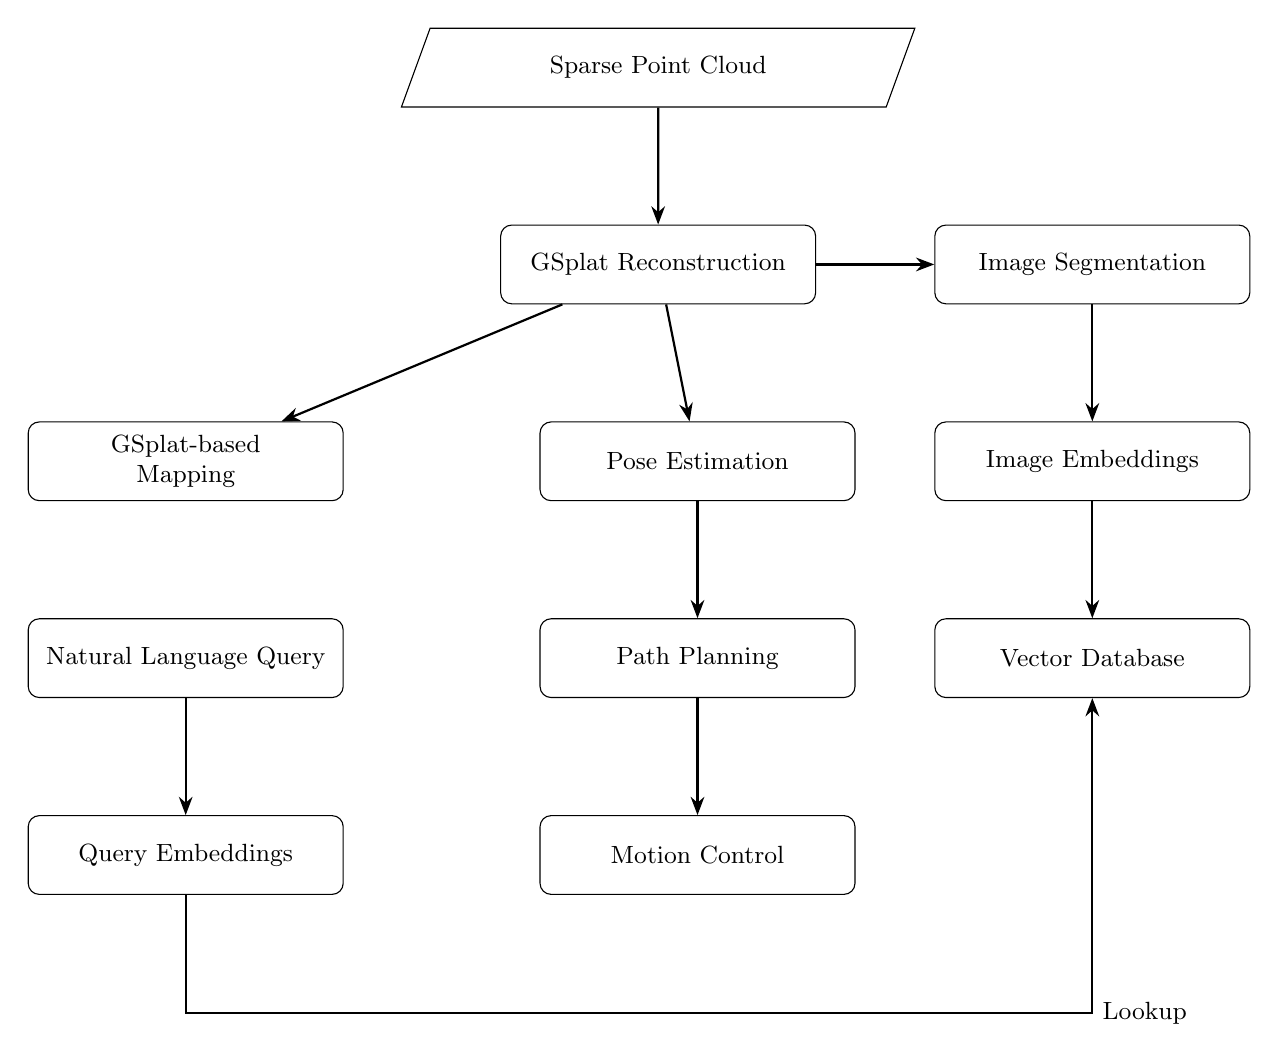
\begin{tikzpicture}[
                  node distance=2.5cm, % Increased node distance
                  every node/.style={font=\small},
                  process/.style={rectangle, draw, minimum width=4cm, minimum height=1cm, rounded corners, align=center},
                  io/.style={trapezium, trapezium left angle=70, trapezium right angle=110, draw, minimum width=4cm, minimum height=1cm, align=center},
                  arrow/.style={thick, ->, >=Stealth}
            ]

            % Nodes
            \node (input) [io] {Sparse Point Cloud};
            \node (reconstruction) [process, below of=input] {GSplat Reconstruction};
            \node (mapping) [process, below of=reconstruction, xshift=-6cm] {GSplat-based\\Mapping}; % Adjusted xshift for more space
            \node (pose) [process, right=0.5cm of reconstruction, below of=reconstruction ] {Pose Estimation}; % Adjusted right shift
            \node (planning) [process, below of=pose] {Path Planning};
            \node (control) [process, below of=planning] {Motion Control};

            % Parallel branch for Image Segmentation, Embeddings, and Vector DB
            \node (segmentation) [process, right=1.5cm of reconstruction] {Image Segmentation}; % Adjusted position
            \node (embedding) [process, below of=segmentation] {Image Embeddings};
            \node (vectorDB) [process, below of=embedding] {Vector Database};

            \node (nlquery) [process, below of=mapping] {Natural Language Query}; % Moved to the bottom left for more space
            \node (nlembedding) [process, below of=nlquery] {Query Embeddings};

            % Arrows
            \draw [arrow] (input) -- (reconstruction);
            \draw [arrow] (reconstruction) -- (pose);
            \draw [arrow] (pose) -- (planning);
            \draw [arrow] (planning) -- (control);
            \draw [arrow] (reconstruction) -- (mapping);

            % Arrows for the parallel branch
            \draw [arrow] (reconstruction) -- (segmentation);
            \draw [arrow] (segmentation) -- (embedding);
            \draw [arrow] (embedding) -- node[anchor=west] {} (vectorDB);

            % Arrows for natural language query
            \draw [arrow] (nlquery) -- (nlembedding);
            \draw [arrow] (nlembedding.south) |- ++(0,-1.5cm) -| node[anchor=west] {Lookup} (vectorDB);

      \end{tikzpicture}
      \caption{GSplat-based Navigation, Mapping, and Semantic Understanding Workflow}
\end{figure}

\section{GSplat-based Navigation and Mapping}

\subsection{GSplat-based Navigation}

\definecolor{codegreen}{rgb}{0,0.6,0}
\definecolor{codegray}{rgb}{0.5,0.5,0.5}
\definecolor{codepurple}{rgb}{0.58,0,0.82}
\definecolor{backcolour}{rgb}{0.95,0.95,0.92}

\lstdefinestyle{mystyle}{
      backgroundcolor=\color{backcolour},
      commentstyle=\color{codegreen},
      keywordstyle=\color{magenta},
      numberstyle=\tiny\color{codegray},
      stringstyle=\color{codepurple},
      basicstyle=\ttfamily\footnotesize,
      breakatwhitespace=false,
      breaklines=true,
      captionpos=b,
      keepspaces=true,
      numbers=left,
      numbersep=5pt,
      showspaces=false,
      showstringspaces=false,
      showtabs=false,
      tabsize=2
}

\lstset{style=mystyle}

\begin{enumerate}
      \item \textbf{GSplat Reconstruction} \\
            Gaussian Splatting initializes the navigation pipeline by transforming a sparse point cloud, obtained via camera calibration or other methods, into 3D Gaussian splats. This reconstruction allows for the environment's geometric representation to be optimized, forming a detailed and efficient basis for real-time navigation tasks. The mathematical representation of a Gaussian splat is given by its mean $\mu \in \mathbb{R}^3$, covariance matrix $\Sigma \in S_{++}$, opacity $\alpha \in [0,1]$, and spherical harmonics coefficients defining view-dependent colors \cite{kerbl20233dgaussiansplattingrealtime}.
            The 3D covariance $\Sigma$ is further decomposed as $\Sigma = R S S^T R^T$, where $R \in SO(3)$ is a rotation matrix and $S$ is a diagonal scaling matrix \cite{chen2024splatnavsaferealtimerobot}.

            To implement the GSplat framework, we utilize a NeRF-based \cite{zhang2024visuallocalization3dmaps} approach provided by
            the `nerfstudio` framework \cite{Tancik_2023}. The following code snippet demonstrates how to
            construct a Gaussian splat model using images from a `data` folder.

            \begin{lstlisting}
      # nerfstudio installation and setup
      pip install nerfstudio
      
      # Prepare your dataset by placing images and camera parameters in the `data` folder
      # The following script initializes the splat model
      
      import nerfstudio as ns
      
      # Path to the dataset
      data_path = "./data"
      
      # Load configuration for the Gaussian Splatting model
      config = ns.configs.get_default_gaussian_splat_config(
            dataset_path=data_path,
            model_name="g_splat_model",
      )
      
      # Instantiate the NeRF Studio pipeline with Gaussian splatting
      pipeline = ns.pipeline.create_pipeline(config)
      
      # Start training the model
      pipeline.train()
      
      # Export the trained splat model for further use in navigation and mapping
      pipeline.save_model("splat_model.pth")
\end{lstlisting}

            This code constructs a Gaussian splatting model from the provided images and
            camera parameters in the `data` folder. The `nerfstudio` framework is leveraged
            to optimize the Gaussian splats for an accurate and efficient environment
            representation. The configuration is automatically managed using the
            \texttt{get\_default\_gaussian\_splat\_config} function, which eliminates the
            need for manual specification of parameters like \texttt{num\_gaussians}.

      \item \textbf{Pose Estimation} \\
            Splat-Loc provides real-time pose estimation by leveraging the point cloud generated from Gaussian splatting. Pose estimation is done using a combination of global initialization and recursive localization based on monocular RGB images. Mathematically, the pose estimation problem can be formulated as a maximum a-posteriori (MAP) optimization problem. Given prior estimates of the robot's pose $\mathbf{x}_{t-1}$ and the measurements $\mathbf{y}_t$, the MAP estimate of the current pose $\mathbf{x}_t$ is computed by minimizing:
            \[
                  \mathbf{x}_t^\star = \arg\min_{\mathbf{x}_t} \left( \| \mathbf{x}_t - f(\mathbf{x}_{t-1}, \mathbf{u}_{t-1}) \|_{Q^{-1}}^2 + \| \mathbf{y}_t - h(\mathbf{x}_t) \|_{R^{-1}}^2 \right)
            \]
            subject to constraints that ensure the pose remains within safe polytope
            corridors defined by the Gaussian splats \cite{bortolon20246dgs6dposeestimation}
            \cite{chen2024splatnavsaferealtimerobot}.

            We are solving the following optimization problem for pose estimation:

            \[
                  x^*_t = \arg \min_{x_t} \left\| x_t - f(x_{t-1}, u_{t-1}) \right\|^2_{Q^{-1}} + \left\| y_t - h(x_t) \right\|^2_{R^{-1}}
            \]

            The Python implementation for this MAP optimization can be written as follows:

            \begin{lstlisting}
import numpy as np
from scipy.optimize import minimize

# Define the state transition function f(x_{t-1}, u_{t-1})
def state_transition(x_prev, u_prev):
    # Example linear transition model
    return np.dot(A, x_prev) + np.dot(B, u_prev)

# Define the measurement function h(x_t)
def measurement_model(x_t):
    # Example measurement model
    return np.dot(C, x_t)

# Define the cost function to minimize
def cost_function(x_t, x_prev, u_prev, y_t, Q_inv, R_inv):
    # State transition error
    state_error = x_t - state_transition(x_prev, u_prev)
    state_cost = np.dot(state_error.T, np.dot(Q_inv, state_error))
    
    # Measurement error
    measurement_error = y_t - measurement_model(x_t)
    measurement_cost = np.dot(measurement_error.T, np.dot(R_inv, measurement_error))
    
    # Total cost
    return state_cost + measurement_cost

# Example matrices (replace with actual values)
A = np.eye(3)  # State transition matrix
B = np.eye(3)  # Control input matrix
C = np.eye(3)  # Measurement matrix
Q_inv = np.eye(3)  # Inverse of process covariance matrix
R_inv = np.eye(3)  # Inverse of measurement covariance matrix

# Previous state, control input, and measurement
x_prev = np.array([1.0, 2.0, 3.0])
u_prev = np.array([0.1, 0.2, 0.3])
y_t = np.array([1.5, 2.5, 3.5])

# Initial guess for the current state
x_t_initial = np.array([1.2, 2.2, 3.2])

# Perform the optimization
result = minimize(cost_function, x_t_initial, args=(x_prev, u_prev, y_t, Q_inv, R_inv))

# Optimal pose estimate
x_t_optimal = result.x
print("Optimal Pose Estimate:", x_t_optimal)
\end{lstlisting}

            This code implements the MAP optimization problem for pose estimation. It uses
            the \texttt{scipy.optimize.minimize} function to find the optimal pose $x_t$ by
            minimizing the cost function, which is a combination of the state transition
            and measurement model errors.

      \item \textbf{Path Planning} \\
            The Splat-Plan module ensures safe navigation through the environment by constructing polytopic safe corridors. These polytopes are created by decomposing the configuration space into occupied and collision-free regions using the intersection of ellipsoidal approximations of the Gaussian splats. The collision-checking algorithm is based on solving generalized eigenvalue problems and can be parallelized for efficiency. Given a set of safe polytopes, the trajectory planning problem is formulated as a quadratic program that minimizes the path length subject to safety constraints:
            \[
                  \min_{\mathbf{c}_i} \sum_{i=0}^{M-1} \|\mathbf{c}_{i+1} - \mathbf{c}_i\|_2^2 \quad \text{subject to } \mathbf{A}\mathbf{c}_i \leq \mathbf{b}
            \]
            where $\mathbf{c}_i$ are the control points of the Bézier curve representing
            the trajectory \cite{chen2024splatnavsaferealtimerobot}.

            The Splat-Plan module ensures safe navigation by constructing polytopic safe
            corridors. These polytopes are created by decomposing the configuration space
            into occupied and collision-free regions using the intersection of ellipsoidal
            approximations of Gaussian splats.

            The trajectory planning problem can be formulated as a quadratic program (QP)
            that minimizes the path length subject to safety constraints:

            \[
                  \min_{\{c_i\}} \sum_{i=0}^{M-1} \left\| c_{i+1} - c_i \right\|^2_2 \quad \text{subject to} \quad A c_i \leq b
            \]

            Here, \( c_i \) are the control points of the Bézier curve representing the
            trajectory. The following Python code implements this optimization problem.

            \begin{lstlisting}
import numpy as np
from scipy.optimize import minimize

# Example quadratic cost function
def trajectory_cost(control_points):
    total_cost = 0
    for i in range(len(control_points) - 1):
        total_cost += np.linalg.norm(control_points[i+1] - control_points[i])**2
    return total_cost

# Example constraint function for the polytope constraints
def polytope_constraints(control_points, A, b):
    constraints = []
    for c_i in control_points:
        constraints.append({'type': 'ineq', 'fun': lambda c_i, A=A, b=b: b - np.dot(A, c_i)})
    return constraints

# Example setup (replace with actual matrices and values)
M = 5  # Number of control points
A = np.array([[1, 0], [0, 1]])  # Example polytope constraint matrix
b = np.array([1, 1])  # Example constraint bounds

# Initial guess for control points (random initialization)
initial_control_points = np.random.rand(M, 2)

# Set up the constraints for all control points
constraints = polytope_constraints(initial_control_points, A, b)

# Perform the optimization (minimizing path length subject to polytope constraints)
result = minimize(trajectory_cost, initial_control_points, constraints=constraints)

# Optimal control points
optimal_control_points = result.x.reshape(M, 2)
print("Optimal Control Points:", optimal_control_points)
\end{lstlisting}

            This code formulates and solves the quadratic program for trajectory planning.
            It minimizes the path length defined by the control points \( c_i \) of a
            Bézier curve, while ensuring that the trajectory remains within the safe
            polytope corridors by enforcing the constraint \( A c_i \leq b \).

      \item \textbf{Motion Control} \\
            The planned trajectory is executed through motion control algorithms that ensure smooth and precise movement of the robot. \cite{DURAKLI2022101540} The trajectory is generated using Bézier curves within the safe polytopes, which guarantees safety and efficiency. The motion control system is integrated with the Gaussian splatting environment, allowing for dynamic adjustments in real-time navigation.

\end{enumerate}

\subsection{GSplat-based Mapping}
\begin{enumerate}
      \item \textbf{GSplat Reconstruction} \\
            For mapping, Gaussian Splatting is used to optimize the representation of 3D Gaussians, which enables efficient storage and real-time updates to the map. The anisotropic covariance matrices are adjusted to balance between map detail and computational efficiency \cite{kerbl20233dgaussiansplattingrealtime}.

      \item \textbf{Exploration and Mapping} \\
            Robots using Gaussian Splatting can perform continuous exploration and mapping, adjusting their internal representation of the environment as they move. The exploration is driven by the robot's need to maintain an updated understanding of the surroundings, avoiding obstacles while generating a detailed map.

      \item \textbf{Map Refinement} \\
            Gaussian splats are refined by adjusting their anisotropic covariances as the robot gathers more data from the environment. This allows for the continuous refinement of the environment representation, ensuring that the robot's map remains accurate and precise over time \cite{kerbl20233dgaussiansplattingrealtime}.

\end{enumerate}

\section{Semantic Understanding and Knowledge Retrieval in GSplat Environments}

The continuous environment representation created by Gaussian splatting is
leveraged for more advanced tasks, including semantic understanding,
image-based query processing, and natural language queries. These processes
enable robots to interact more meaningfully with their surroundings by
providing both perceptual and cognitive capabilities.\cite{che2024enhancingmultimodalunderstandingclipbased}

\subsection{Image Segmentation and Embeddings}

After the environment has been reconstructed using Gaussian splatting, the
robot performs image segmentation to identify objects and regions of interest
within its field of view. Image segmentation divides the visual input into
segments corresponding to distinct objects or surfaces, helping the robot to
parse the environment into meaningful components. \cite{ravi2024sam}

Once the image segmentation process is complete, the segmented regions are
passed through a neural network to generate high-dimensional image embeddings.
These embeddings represent the visual content in a compact form, capturing the
essential features of each segment. The embeddings are crucial for both object
recognition and later retrieval tasks. \cite{che2024enhancingmultimodalunderstandingclipbased}

\begin{figure}[h]
      \centering
      \includegraphics[width=\textwidth]{embeddings.png} % Adjust the width as necessary
      \caption{Image Embeddings for Semantic Understanding} % Caption for the image
      \label{fig:embeddings} % Label for referencing the image
\end{figure}

\subsection*{1. Convert Image to Embeddings}

We use the CLIP model from the `transformers` library to convert images into
embeddings.

\begin{lstlisting}
from transformers import CLIPProcessor, CLIPModel
from PIL import Image
import torch

# Load a pre-trained CLIP model and processor
model = CLIPModel.from_pretrained("openai/clip-vit-base-patch32")
processor = CLIPProcessor.from_pretrained("openai/clip-vit-base-patch32")

# Function to convert an image to embeddings
def image_to_embeddings(image_path):
    image = Image.open(image_path)
    inputs = processor(images=image, return_tensors="pt")
    with torch.no_grad():
        embeddings = model.get_image_features(**inputs)
    return embeddings.squeeze().numpy()

# Example usage
image_path = "example_image.jpg"
image_embeddings = image_to_embeddings(image_path)
print("Image Embeddings:", image_embeddings)
\end{lstlisting}

\subsection*{2. Store Embeddings in ChromaDB}

After converting the image to embeddings, we store the embeddings in ChromaDB which uses FAISS  to lookup similar embeddings efficiently. \cite{douze2024faisslibrary},
a vector database for efficient storage and retrieval of embeddings.

\begin{lstlisting}
import chromadb
from chromadb.utils import embedding_store

# Initialize ChromaDB client
client = chromadb.Client()

# Create a collection to store embeddings
collection = client.create_collection("multimodal_embeddings")

# Function to store embeddings in ChromaDB
def store_embeddings(id, embeddings, metadata=None):
    collection.add(id=id, embedding=embeddings.tolist(), metadata=metadata)

# Store the image embeddings with an identifier
store_embeddings(id="image_1", embeddings=image_embeddings, metadata={"type": "image"})
\end{lstlisting}

\subsection*{3. Convert Text Query to Embeddings}

We convert a text query into embeddings using the same CLIP model, allowing for
multimodal comparisons. \cite{che2024enhancingmultimodalunderstandingclipbased}

\begin{lstlisting}
# Function to convert text query to embeddings
def text_to_embeddings(text_query):
    inputs = processor(text=text_query, return_tensors="pt")
    with torch.no_grad():
        embeddings = model.get_text_features(**inputs)
    return embeddings.squeeze().numpy()

# Example usage
text_query = "A cat sitting on a chair"
text_embeddings = text_to_embeddings(text_query)
print("Text Query Embeddings:", text_embeddings)
\end{lstlisting}

\subsection{Vector Database Lookup}

The image embeddings generated from the segmented regions are stored in a
vector database along with their associated locations in the point cloud. The
vector database enables fast and efficient retrieval of similar embeddings,
facilitating object recognition, tracking, and semantic labeling.

During navigation, if the robot encounters a previously observed region or
object, it can perform a vector database lookup by comparing the current image
embeddings with the stored embeddings. This comparison allows the robot to
recognize familiar objects and recall their previously associated semantic
labels, enabling context-aware decision-making and interaction with the
environment.\cite{douze2024faisslibrary}

\begin{lstlisting}
      # Function to lookup similar embeddings in ChromaDB
      def query_similar_embeddings(embeddings, top_k=5):
          results = collection.query(embedding=embeddings.tolist(), n_results=top_k)
          return results
      
      # Query similar embeddings using the text query embeddings
      similar_embeddings = query_similar_embeddings(text_embeddings)
      print("Similar Embeddings:", similar_embeddings)
      \end{lstlisting}

\subsection{Natural Language Query Processing}

In addition to image-based processing, the robot is capable of understanding
and processing natural language queries. The process begins with the robot
receiving a natural language query, such as "Where is the nearest charging
station?" or "Identify the red object in the room."

The query is first converted into a high-dimensional embedding using a
pre-trained language model. This embedding captures the meaning of the query
and is used to perform a semantic lookup in the vector database. The robot
compares the query embedding with the stored image embeddings and retrieves the
relevant objects or locations that match the query.

For example, if the query is about finding a specific object, the robot will
locate the corresponding image embeddings in the vector database and return the
object's location in the point cloud. This allows the robot to answer questions
about its environment and provide meaningful responses based on its prior
knowledge and observations. \cite{che2024enhancingmultimodalunderstandingclipbased}

\subsection{Integration with Navigation and Mapping}

The semantic understanding and query processing capabilities are integrated
with the GSplat-based navigation and mapping pipeline. As the robot explores
its environment, it continuously updates its internal representation with new
Gaussian splats, image embeddings, and semantic labels. This enables the robot
to build a rich and detailed map of the environment that can be queried both
visually and linguistically.

Furthermore, the vector database provides a way to efficiently store and
retrieve this information, allowing the robot to recognize objects and
locations that it has previously encountered. This integration ensures that the
robot can perform advanced navigation tasks while maintaining an updated
understanding of its surroundings.

By combining Gaussian splatting with image segmentation, embeddings, and
natural language processing, the robot can achieve a high level of semantic
understanding, enabling it to interact with complex environments in a
meaningful and intelligent way.



\chapter{Image-Based Disease and Pest Detection}

The detection of plant diseases and pests is a critical task in agriculture, as
early identification can prevent widespread crop damage and reduce yield
losses. Traditional methods of disease detection rely on visual inspection by
human experts, which can be time-consuming and subjective. In recent years, the
application of deep learning techniques, particularly convolutional neural
networks (CNNs), has shown promising results in automating the detection of
plant diseases from images. This chapter explores the use of CNNs for
image-based disease and pest detection in crops, focusing on the dataset, model
architecture, training process, and performance evaluation.\cite{10.3389/fpls.2016.01419}

\begin{figure}[h!]
    \centering
    \includegraphics[width=0.8\textwidth]{cnn_architecture_diagram.png}
    \caption{Convolutional Neural Network (CNN) Architecture for Disease Detection.}
    \label{fig:cnn_architecture}
\end{figure}

\section{Dataset}
The model is trained on the PlantVillage dataset, which contains 54,306 images
of plant leaves categorized into 38 classes, representing both healthy and
diseased leaves across various crops. The images are resized to 256x256 pixels
for input into the CNN model. \cite{J2019}

\subsection{Preprocessing}
Before feeding the images into the model, they are preprocessed to enhance the
training efficiency. Preprocessing steps include resizing, normalization, and
data augmentation techniques such as rotation, zoom, and flipping to improve
the model's robustness. \cite{yim2021plantdiseasedetection}

\section{Model Architecture}
The proposed method employs a CNN architecture, which consists of multiple
convolutional layers, max-pooling layers, and fully connected layers. The
architecture extracts features from the input images and classifies them into
healthy or diseased categories.

\subsection{Convolutional Layers}
Convolutional layers are the foundation of CNNs. Each convolutional layer
applies filters to the input images to detect specific features, such as edges,
textures, and patterns. \cite{oshea2015introductionconvolutionalneuralnetworks}

\subsection{Pooling Layers}
Pooling layers perform down-sampling operations to reduce the spatial
dimensions of the feature maps. Max pooling is the most commonly used
technique, where the maximum value within a sliding window is selected.

\subsection{Fully Connected Layers}
After feature extraction, fully connected layers map the features to output
classes representing different plant diseases.

\section{Training and Evaluation}
The CNN model is trained using the PlantVillage dataset with 80\% of the data
used for training and 20\% for testing. The model is optimized using the Adam
optimizer, and the categorical cross-entropy loss function is employed. The
training process is carried out for ten epochs.

\subsection{Performance Metrics}
The model's performance is evaluated using accuracy and loss metrics. The
trained model achieves an accuracy of 95\% on the training data and 94\% on the
test data, demonstrating its effectiveness in classifying plant diseases.

\section{Fine-tuning the Model}
Fine-tuning is an essential step in improving the model's accuracy by
leveraging pre-trained models. Below is an example of fine-tuning a pre-trained
CNN model (e.g., VGG16) on the PlantVillage dataset. \cite{radenović2018finetuningcnnimageretrieval}

\begin{lstlisting}[language=Python, caption=Fine-tuning a Pre-trained CNN]
from tensorflow.keras.applications import VGG16
from tensorflow.keras.preprocessing.image import ImageDataGenerator
from tensorflow.keras.layers import Dense, Flatten
from tensorflow.keras.models import Model
from tensorflow.keras.optimizers import Adam

# Load the pre-trained VGG16 model
base_model = VGG16(weights='imagenet', include_top=False, input_shape=(256, 256, 3))

# Freeze the layers of the pre-trained model
for layer in base_model.layers:
    layer.trainable = False

# Add custom layers on top of the base model
x = Flatten()(base_model.output)
x = Dense(128, activation='relu')(x)
x = Dense(64, activation='relu')(x)
predictions = Dense(38, activation='softmax')(x)

# Define the final model
model = Model(inputs=base_model.input, outputs=predictions)

# Compile the model
model.compile(optimizer=Adam(learning_rate=0.0001), loss='categorical_crossentropy', metrics=['accuracy'])

# Data augmentation
train_datagen = ImageDataGenerator(rescale=1./255, rotation_range=20, width_shift_range=0.2, height_shift_range=0.2, horizontal_flip=True)
test_datagen = ImageDataGenerator(rescale=1./255)

# Load training and testing data
train_generator = train_datagen.flow_from_directory('data/train', target_size=(256, 256), batch_size=32, class_mode='categorical')
test_generator = test_datagen.flow_from_directory('data/test', target_size=(256, 256), batch_size=32, class_mode='categorical')

# Train the model
history = model.fit(train_generator, epochs=10, validation_data=test_generator)

# Evaluate the model
loss, accuracy = model.evaluate(test_generator)
print(f'Test Accuracy: {accuracy * 100:.2f}%')
\end{lstlisting}

% \chapter{Harvest State Detection Using Image Models}
This section discusses how image models are used to determine the optimal harvest time for crops. By analyzing images of crops, these models can assess factors such as ripeness, size, and color to provide accurate harvest timing recommendations.

\section{Image Analysis Techniques}
\subsection{Color-Based Analysis}
\subsection{Shape and Size Detection}
\subsection{Texture Analysis}

\section{Model Training and Validation}
\subsection{Dataset Preparation}
\subsection{Training Procedures}
\subsection{Validation and Testing}

\chapter{Large Language Models (LLM) for Agricultural Task Planning}
\section{Multi-Agent Coordination}
\section{Task Planning}
\section{Tool Usage}
\section{Information Extraction and Continuous Learning}

\chapter{Visual Language Action Models (VLAMs) for Agricultural Robotics}

\section{Integration with Robotic Control}
OpenVLA integrates pre-trained vision-language models (VLMs) \cite{kim2024openvlaopensourcevisionlanguageactionmodel} for controlling agricultural robots. By building on a Llama 2 \cite{touvron2023llamaopenefficientfoundation} backbone combined with visual encoders from DINOv2 and SigLIP, OpenVLA allows the mapping of visual input $\mathbf{I}$ and language instructions $\mathbf{L}$ to robot control actions $\mathbf{A}$.

Let $\mathbf{I}$ be the input image from the robot's camera and $\mathbf{L}$ be the language instruction provided by the user. The model predicts the robot's action $\mathbf{A}$ by performing the following operation:
\[
\mathbf{A} = \text{VLA}(\mathbf{I}, \mathbf{L}),
\]
where $\text{VLA}$ represents the vision-language-action model, which outputs the robot's control actions, such as gripper position, orientation, and grip force.

The architecture of OpenVLA is shown in Figure \ref{fig:openvla_architecture}, where visual features from DINOv2 and SigLIP are concatenated and projected into the input space of the Llama 2 language model. The language model then generates robot actions in the form of discrete tokens.

\begin{figure}[h]
\centering
\includegraphics[width=0.8\textwidth]{openvla.png}
\caption{OpenVLA model architecture. The visual encoder extracts features from the input image, which are concatenated and projected into the input space of the Llama 2 language model. The model then generates robot control actions.}
\label{fig:openvla_architecture}
\end{figure}

For practical deployment, the OpenVLA model can be served over a REST API, enabling seamless integration with robotic control systems in real-time. The code snippet below demonstrates deploying OpenVLA models via a lightweight server using the HF AutoClass API:

\begin{lstlisting}[language=Python, caption=OpenVLA Deployment Server Example]
import os.path
import json_numpy
json_numpy.patch()
import json
import logging
import traceback
from pathlib import Path
from typing import Any, Dict, Optional, Union

import torch
import uvicorn
from fastapi import FastAPI
from PIL import Image
from transformers import AutoModelForVision2Seq, AutoProcessor

class OpenVLAServer:
    def __init__(self, openvla_path: Union[str, Path]):
        self.device = torch.device("cuda:0" if torch.cuda.is_available() else "cpu")
        self.processor = AutoProcessor.from_pretrained(openvla_path, trust_remote_code=True)
        self.vla = AutoModelForVision2Seq.from_pretrained(
            openvla_path, torch_dtype=torch.bfloat16, low_cpu_mem_usage=True, trust_remote_code=True
        ).to(self.device)

    def predict_action(self, payload: Dict[str, Any]) -> str:
        image, instruction = payload["image"], payload["instruction"]
        inputs = self.processor(instruction, Image.fromarray(image).convert("RGB")).to(self.device, dtype=torch.bfloat16)
        action = self.vla.generate(**inputs)
        return action

    def run(self, host: str = "0.0.0.0", port: int = 8000):
        app = FastAPI()
        app.post("/act")(self.predict_action)
        uvicorn.run(app, host=host, port=port)

if __name__ == "__main__":
    server = OpenVLAServer("path_to_model")
    server.run()
\end{lstlisting}

\section{Co-Fine-Tuning}
OpenVLA supports efficient fine-tuning on new agricultural tasks using small datasets. The model leverages modern parameter-efficient techniques such as Low-Rank Adaptation (LoRA), which allows fine-tuning only a small percentage of the model parameters while maintaining performance \cite{hu2021lora}. 

The fine-tuning objective can be written as minimizing the cross-entropy loss $\mathcal{L}_{CE}$ between the predicted token sequence $\hat{\mathbf{T}} = \{\hat{t}_1, \hat{t}_2, \dots, \hat{t}_n\}$ and the ground truth token sequence $\mathbf{T} = \{t_1, t_2, \dots, t_n\}$, representing the robot actions:
\[
\mathcal{L}_{CE}(\hat{\mathbf{T}}, \mathbf{T}) = -\sum_{i=1}^{n} t_i \log(\hat{t}_i).
\]
During fine-tuning, the model updates its parameters $\theta$ by optimizing the following loss function:
\[
\theta^* = \arg \min_\theta \mathbb{E}_{(\mathbf{I}, \mathbf{L}, \mathbf{T}) \sim \mathcal{D}} \left[\mathcal{L}_{CE}(\hat{\mathbf{T}}, \mathbf{T})\right],
\]
where $\mathcal{D}$ represents the dataset of image-language-action triplets.

\section{Action as Text Tokens}
The OpenVLA model maps continuous robot actions into discrete tokens using the Llama 2 tokenizer \cite{touvron2023llamaopenefficientfoundation}. The robot actions, $\mathbf{A}$, are first discretized into $K$ bins per dimension, resulting in a sequence of discrete tokens $\mathbf{T}$:
\[
\mathbf{T} = \text{Discretize}(\mathbf{A}) = \{t_1, t_2, \dots, t_n\},
\]
where $t_i \in \{0, 1, \dots, K-1\}$.

The token sequence is then processed by the language model to predict the next action in a sequence-to-sequence manner\cite{sutskever2014sequencesequencelearningneural}. The final action $\hat{\mathbf{A}}$ is reconstructed by decoding the predicted tokens:
\[
\hat{\mathbf{A}} = \text{Decode}(\hat{\mathbf{T}}).
\]

This approach allows the model to handle agricultural tasks such as precise gripper positioning and adjusting the robot arm's trajectory based on the environment.

\section{Real-Time Inference}
Real-time inference is crucial for agricultural robotics, where decisions need to be made instantly based on sensor inputs. OpenVLA's remote inference solution, released as part of the codebase, supports streaming of action predictions to agricultural robots in real-time.

The latency of the inference process can be represented as:
\[
\text{Latency} = T_{\text{preprocess}} + T_{\text{forward}} + T_{\text{postprocess}},
\]
where $T_{\text{preprocess}}$ is the time taken to preprocess the input image and text, $T_{\text{forward}}$ is the forward pass through the model, and $T_{\text{postprocess}}$ is the time taken to convert the predicted tokens back into actions.


\section{Generalization and Emergent Capabilities}
OpenVLA demonstrates strong generalization capabilities across diverse agricultural tasks, such as handling unseen crops, varying lighting conditions, and multiple objects in complex environments. The model's ability to generalize is a result of both the large-scale Internet-pretrained data and the fine-tuning on agricultural-specific datasets.

The model's generalization can be evaluated by its performance on unseen tasks, which is quantified by the success rate $S$:
\[
S = \frac{\text{Number of successful task completions}}{\text{Total number of task attempts}}.
\]
OpenVLA achieves high success rates across a wide range of agricultural tasks, demonstrating its robustness and adaptability.

The emergence of such capabilities in VLAMs is attributed to the combination of large-scale Internet-pretrained data and task-specific fine-tuning, which allows for learning transferable skills across different agricultural domains.




\chapter{Agricultural Robot System}

This chapter describes the design and functioning of an agricultural robot that autonomously navigates, detects diseases and pests, and sprays chemicals using advanced technologies such as Gaussian splatting and convolutional neural networks (CNNs). The robot is constructed with aluminum extrusion as its frame, motors for movement and arm control, and various sensors and components for navigation and operation. An Android application is used to control both the Arduino Uno and the ESP32 microcontrollers for precise movement and spraying actions.

\section{System Overview}

The robot uses a mobile phone, specifically a Google Pixel, as its primary processing unit. \cite{müller2021openbotturningsmartphonesrobots} The phone's camera captures images to create a 3D Gaussian splat map for navigation, allowing the robot to identify its position in the field and locate target objects for spraying. Additionally, the robot is capable of identifying diseases and pests using a CNN-based model trained on agricultural datasets. The system operates as follows:

\begin{enumerate}
    \item The robot wakes up and captures an image using the phone's camera.
    \item The image is processed to create a 3D Gaussian splat for localization and mapping.\cite{chen2024splatnavsaferealtimerobot} \cite{bortolon20246dgs6dposeestimation}
    \item Simultaneously, the image is analyzed using a CNN-based model to detect diseases or pests on plants.\cite{10353343}
    \item Based on the identified location and any detected issues, the robot receives instructions to move to a specific point.\cite{DURAKLI2022101540}
    \item Using OpenVLA, the robot performs actions such as moving its arms and spraying chemicals on the target objects. \cite{kim2024openvlaopensourcevisionlanguageactionmodel}
\end{enumerate}

The system connects to the web server to send images, receive instructions for navigation, and apply actions based on disease and pest identification. An Android application is also used to control the robot’s movement and spraying mechanism, providing a user-friendly interface for manual control when needed.

\section{Communication and Control}
The Android phone uses USB-C to serial adapter to communicate with the Arduino Uno and ESP32 microcontrollers. The Arduino Uno controls the motors for arm movement and the hydraulic motor for spraying, while the ESP32 controls the base wheel motors for navigation. The phone captures images and sends them to the cloud server for processing, receiving navigation instructions and action tokens in return. The robot's operation is coordinated through a combination of image processing, navigation algorithms, and disease/pest detection logic.


\section{Gaussian Splatting for Navigation and Mapping}

Gaussian splatting offers an innovative approach to real-time navigation, mapping, and semantic understanding by transforming sparse 3D point clouds into continuous Gaussian distributions (splats). This technique provides an efficient representation of the environment, enabling the robot to perform real-time updates and optimizations for navigation tasks.

The key components of Gaussian splatting include:
\begin{itemize}
    \item \textbf{GSplat Reconstruction:} The robot converts images captured by the camera into 3D Gaussian splats, forming a geometric representation of the environment. This allows the robot to optimize navigation in real-time. \cite{chen2024splatnavsaferealtimerobot}
    \item \textbf{Pose Estimation:} Using the Gaussian splat map, the robot performs pose estimation to accurately determine its position in the field. \cite{bortolon20246dgs6dposeestimation}
    \item \textbf{Path Planning:} The robot plans its path by constructing polytopic safe corridors, ensuring collision-free navigation.\cite{DURAKLI2022101540}
    \item \textbf{Motion Control:} The planned trajectory is executed through smooth motion control, integrated with the Gaussian splat environment for dynamic adjustments during navigation.\cite{DURAKLI2022101540}
\end{itemize}

This approach enables the robot to navigate autonomously in complex agricultural environments, continuously refining its internal map as it moves through the field.


\section{Electronics and Control System}

The robot's electronics are controlled by an Arduino Uno, which drives the motors in the arms. The power system consists of an S4 9V battery, which is converted to 12V using a voltage converter. The motor control is achieved using TMC2208 drivers, providing smooth and precise control of the arm motors.

The base wheel motors are powered by a separate battery, identical to the one used for the arms. The ESP32 microcontroller, along with a relay, controls the motors and ensures proper movement of the robot. The hydraulic motor for the spraying mechanism is also controlled by the Arduino Uno.

\section{Hydraulic System}
The hydraulic system of the robot consists of a pump, a reservoir, and a spraying mechanism. The pump is powered by a separate power supply, providing the necessary pressure to drive the liquid spraying system. The reservoir holds the chemicals to be sprayed, which are released through the spraying mechanism when activated. The hydraulic system is controlled by the Arduino Uno, ensuring precise and efficient spraying of chemicals on target objects.

\cite{azghadi2024preciseroboticweedspotspraying}

\subsection{Power System}

The power system of the robot consists of:

\begin{itemize}
    \item An S4 9V battery for the arm motors and control system.
    \item A voltage converter to step up the voltage to 12V for motor operation.
    \item TMC2208 motor drivers to control the NEMA 17 motors.
    \item A separate S4 9V battery for the base wheel motors.
    \item Power supply for the hydraulic motor to drive the liquid spraying system.
    \item Hydraulic pump and reservoir for chemical spraying using a Relay.
\end{itemize}

\section{Software and Communication}

The robot's software is based on a combination of image processing, navigation algorithms, disease/pest detection, and motor control logic. The mobile phone serves as the main computational brain, performing the following tasks:

\begin{itemize}
    \item Capturing images for localization and disease/pest detection.
    \item Sending images to the cloud server to create a 3D Gaussian splat map.
    \item Analyzing images using the CNN model to detect diseases and pests.
    \item Receiving instructions from the server based on the identified location and detected issues.
    \item Using OpenVLA to generate action tokens for arm movement and spraying.
\end{itemize}

The ESP32 microcontroller is responsible for controlling the base motors, using feedback from an accelerometer to maintain stability and ensure accurate navigation. The Android application provides manual control over the robot, enabling the user to issue movement commands or activate the spraying mechanism when needed.

\section{Operation Workflow}

The robot operates autonomously in the field with the following workflow:

\begin{enumerate}
    \item The robot powers on and initializes all systems.
    \item The mobile phone captures an image of the surroundings.
    \item The image is sent to the cloud server for localization using Gaussian splatting.
    \item Simultaneously, the image is analyzed for disease and pest detection using a CNN model.
    \item The robot receives navigation instructions and moves to the specified location.
    \item The arms are positioned based on action tokens generated by OpenVLA.
    \item The spraying mechanism is activated using the hydraulic motor, and chemicals are applied to the target object if diseases or pests are detected.
    \item The user can also manually control the robot's movement and spraying mechanism using the Android app.
\end{enumerate}

\section{IK and FK for Arm Movement}

The robot's arm movement is controlled using Inverse Kinematics (IK) and Forward Kinematics (FK) algorithms. The IK algorithm calculates the joint angles required to position the end effector at a specific location, while the FK algorithm determines the end effector's position based on the joint angles. These algorithms enable precise and efficient control of the robot's arms, allowing it to perform complex tasks such as spraying chemicals on target objects.
Using a grid based system with the image segmentation, the robot can identify the location of the target object and calculate the IK and FK to move the arm to the desired position.


\section{Workflow Diagram}

\begin{figure}[h]
    \centering
    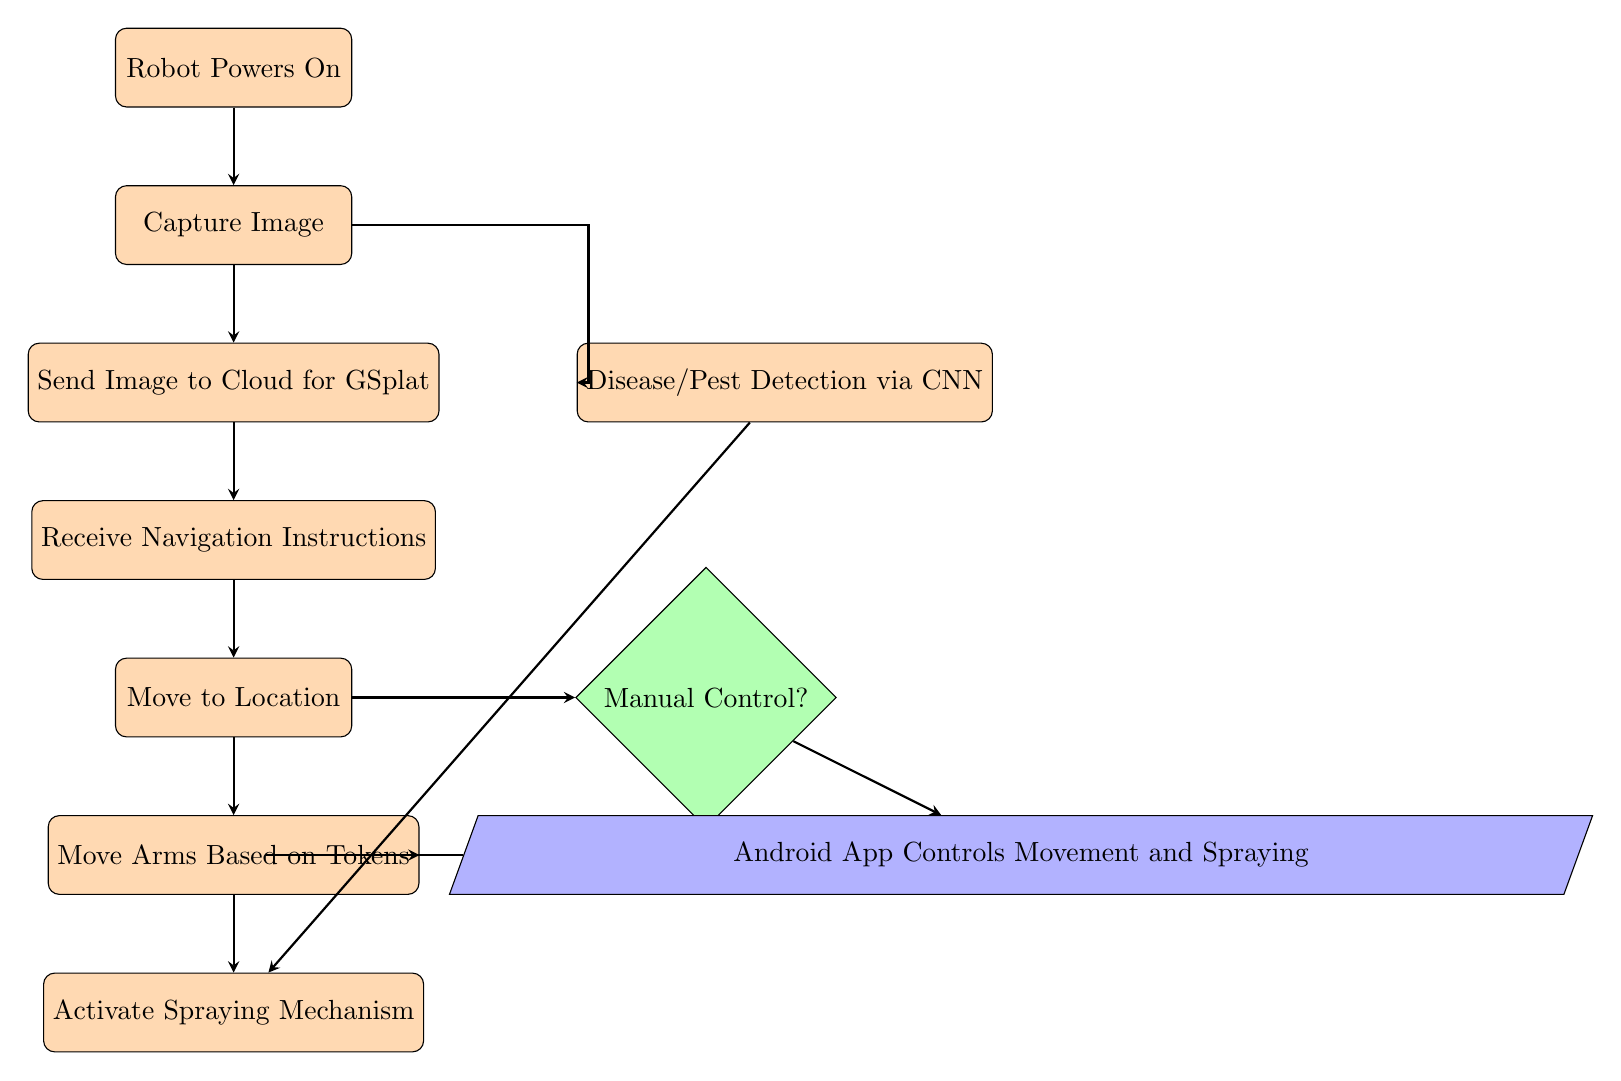
\begin{tikzpicture}[node distance=2cm]
        % Define block styles
        \tikzstyle{process} = [rectangle, rounded corners, minimum width=3cm, minimum height=1cm, text centered, draw=black, fill=orange!30]
        \tikzstyle{decision} = [diamond, minimum width=3cm, minimum height=1cm, text centered, draw=black, fill=green!30]
        \tikzstyle{io} = [trapezium, trapezium left angle=70, trapezium right angle=110, minimum width=3cm, minimum height=1cm, text centered, draw=black, fill=blue!30]
        \tikzstyle{arrow} = [thick,->,>=stealth]
        
        % Nodes
        \node (start) [process] {Robot Powers On};
        \node (image) [process, below of=start] {Capture Image};
        \node (cloud) [process, below of=image] {Send Image to Cloud for GSplat};
        \node (detection) [process, right of=cloud, xshift=5cm] {Disease/Pest Detection via CNN};
        \node (server) [process, below of=cloud] {Receive Navigation Instructions};
        \node (move) [process, below of=server] {Move to Location};
        \node (arms) [process, below of=move] {Move Arms Based on Tokens};
        \node (spray) [process, below of=arms] {Activate Spraying Mechanism};
        
        \node (manual) [decision, right of=move, xshift=4cm] {Manual Control?};
        \node (android) [io, below of=manual, xshift=4cm] {Android App Controls Movement and Spraying};
        
        % Arrows
        \draw [arrow] (start) -- (image);
        \draw [arrow] (image) -- (cloud);
        \draw [arrow] (cloud) -- (server);
        \draw [arrow] (server) -- (move);
        \draw [arrow] (move) -- (arms);
        \draw [arrow] (arms) -- (spray);
        
        \draw [arrow] (image.east) -- ++(3,0) |- (detection);
        \draw [arrow] (detection) -- (spray);
        
        \draw [arrow] (move.east) -- ++(1.5,0) |- (manual);
        \draw [arrow] (manual) -- (android);
        \draw [arrow] (android.west) -- ++(-2.5,0) |- (arms);
    \end{tikzpicture}
    \caption{Workflow of the Agricultural Robot System}
\end{figure}

\begin{figure}[h]
    \centering
    \includegraphics[width=0.8\textwidth]{robot.png}
    \caption{Diagram of the Agricultural Robot}
\end{figure}

\begin{figure}[h]
    \centering
    \includegraphics[width=0.8\textwidth]{legs.png}
    \caption{Wheels of the Agricultural Robot}
\end{figure}

\begin{figure}[h]
    \centering
    \includegraphics[height=0.3\textwidth]{arm.png}
    \caption{Arm of the Agricultural Robot}
\end{figure}

\section{Tools Used}

The following tools were used in the development of the agricultural robot system:

\begin{itemize}
    \item \textbf{Arduino Uno:} Controls the arm motors and hydraulic motor.
    \item \textbf{ESP32:} Controls the base wheel motors for navigation.
    \item \textbf{Google Pixel:} Acts as the main processing unit for image capture and analysis.
    \item \textbf{Android App:} Provides manual control over the robot's movement and spraying mechanism.
    \item \textbf{OpenVLA:} Generates action tokens for arm movement and spraying based on visual and language inputs.
    \item \textbf{Gaussian Splatting:} Creates a 3D Gaussian splat map for navigation and mapping.
    \item \textbf{CNN Model:} Detects diseases and pests in plants from captured images.
    \item \textbf{Hydraulic System:} Sprays chemicals on target objects based on detected issues.
    \item \textbf{IK and FK Algorithms:} Control the arm movement for precise positioning.
    \item \textbf{Grid Based System:} Identifies the location of target objects for arm movement.
    \item \textbf{Image Segmentation:} Analyzes images to detect diseases and pests in plants.
    \item \textbf{Web Server:} Communicates with the robot to provide navigation instructions and action tokens.
    \item \textbf{Voltage Converter:} Steps up the voltage to 12V for motor operation.
    \item \textbf{TMC2208 Motor Drivers:} Control the NEMA 17 motors for smooth and precise movement.
    \item \textbf{Relay:} Controls the hydraulic motor for spraying chemicals on target objects.
    \item \textbf{Accelerometer:} Provides feedback for maintaining stability during navigation.
    \item \textbf{CAD - Onshape} Used for designing the robot and its components.
    \item \textbf{Python:} Programming language used for developing the robot's software.
    \item \textbf{FastAPI:} Web framework used for creating the REST API for communication.
    \item \textbf{Orca Slicer:} Used for slicing the 3D models for printing.
    \item \textbf{Ender 3:} 3D printer used for printing the robot's components.
    \item \textbf{S4 9V Battery:} Power source for the arm motors and control system.

\end{itemize}


\chapter{Conclusion}

The agricultural sector is undergoing a transformative phase, driven by the integration of advanced technologies such as robotics, spatial mapping, and multi-modal language models. This report has explored how these technologies, when applied effectively, can revolutionize traditional farming practices and address the pressing challenges faced by modern agriculture, such as climate change, resource scarcity, and the growing global demand for food.

One of the central contributions of this research has been the application of Gaussian splatting for real-time navigation and mapping in agricultural environments. By transforming sparse 3D point clouds into continuous Gaussian distributions, this method provides a precise and efficient representation of the environment. The ability of agricultural robots to navigate through complex terrains with safety and accuracy is greatly enhanced by this technique. Gaussian splatting also supports dynamic real-time updates, allowing robots to continually refine their understanding of the environment as they move through it. This level of precision in navigation is crucial for autonomous farming systems, where the ability to make real-time decisions can lead to more efficient field operations and reduce the margin of error in crop management.

Another major focus of this report has been on the use of convolutional neural networks (CNNs) for disease and pest detection in crops. The CNN-based models trained on agricultural datasets have demonstrated their effectiveness in accurately identifying diseases and pests from plant images. This capability is vital for precision agriculture, as it allows for targeted interventions that can prevent widespread crop damage, reduce the unnecessary use of pesticides, and promote healthier crop growth. By leveraging CNNs, farmers can move away from traditional blanket spraying techniques and instead adopt a more focused approach that conserves resources and minimizes environmental impact.

In addition to these advancements, the integration of Visual Language Action Models (VLAMs) into agricultural robotics represents a significant leap forward. VLAMs allow robots to interpret and respond to natural language instructions in combination with visual data, enabling them to perform complex tasks autonomously. For example, a robot equipped with VLAM capabilities can navigate a field, identify specific crops, and execute actions such as spraying pesticides or applying fertilizers based on spoken commands. This integration of language and vision into robotic control systems enhances the versatility and adaptability of agricultural robots, allowing them to handle a wider range of tasks with minimal human intervention.

While the current system shows significant promise, several areas for improvement have been identified. The following improvements could enhance the performance and efficiency of the system:

\begin{itemize}
    \item \textbf{Onboard Computer:} The system would benefit from the inclusion of an onboard computer with sufficient computational power to run the necessary models directly on the robot. Currently, the processing relies heavily on external systems, which introduces latency and reduces real-time responsiveness. An onboard computer would enhance autonomy and reduce dependency on cloud-based infrastructure, allowing for quicker decision-making and more efficient operations in the field.
    \item \textbf{Wheelbase Optimization:} The robot's current wheelbase design is not optimal for navigating farm environments. \cite{Elsheikh2023} The existing design struggles with uneven terrain and lacks the necessary stability for consistent performance in rough agricultural settings. A track-based system with suspension would provide better traction, stability, and adaptability to the varying conditions found in farms, leading to improved navigation and task execution.
    \item \textbf{Frame Sturdiness:} The robot's frame, currently constructed from aluminum extrusion, has shown weaknesses under the demands of field operation. Replacing the frame with a more robust core material could significantly improve the robot's durability and longevity. A sturdier frame would better withstand the stresses of farm work, especially when carrying heavy equipment or operating in harsh conditions.
\end{itemize}

The implications of these findings are far-reaching. The successful integration of robotics, spatial mapping, and language models into agriculture can lead to significant improvements in productivity, sustainability, and cost-efficiency. Autonomous robots equipped with advanced perception and decision-making capabilities can perform repetitive and labor-intensive tasks, freeing up human labor for more strategic activities. Moreover, by optimizing the use of inputs such as water, fertilizers, and pesticides, these technologies can contribute to more sustainable farming practices that are better aligned with environmental conservation goals.

Despite the promising results, this research also highlights areas where further exploration is needed. The future of agricultural robotics will depend on continuous improvements in several key areas. First, advancements in real-time data processing and the development of more robust algorithms will be essential to ensure that robots can operate effectively in diverse and unpredictable agricultural environments. Second, the availability of larger and more diverse datasets for disease and pest detection will be critical in improving the accuracy and generalization capabilities of CNN models.\cite{cieslak2024generatingdiverseagriculturaldata} As agricultural environments vary widely across regions and climates, models must be trained on data that reflect this diversity to be effective on a global scale.

Furthermore, the generalization capabilities of Visual Language Action Models must be enhanced to handle more complex and nuanced instructions, especially in multilingual and culturally diverse farming contexts. Fine-tuning these models for specific agricultural tasks while ensuring they maintain their adaptability to new tasks is an ongoing challenge. Additionally, as these technologies continue to develop, ethical considerations such as data privacy, the impact on rural employment, and the equitable distribution of technological benefits must be addressed to ensure that the advancements in agricultural robotics contribute positively to society as a whole.

In conclusion, the combination of robotics, spatial mapping, and multi-modal language models holds immense potential for the future of agriculture. By continuing to innovate in these areas, we can create more efficient, resilient, and sustainable farming systems that are capable of meeting the demands of a growing global population. This research marks an important step toward realizing that vision, but there is still much work to be done. As we move forward, the integration of cutting-edge technologies into agriculture will require a collaborative effort from researchers, engineers, farmers, and policymakers to ensure that these advancements are implemented in ways that maximize their benefits for both people and the planet.




\bibliographystyle{plain}
\bibliography{references}


\end{document}
